\section{実験手順}
本研究の実験の流れを説明する.実験1回ごとの機械学習フローを図\ref{fig:ml-flow}に示す.
これは予め用意されたデータセットと,検証内容に応じて設定された条件設定を入力として,精度を出力するまでの一連の流れである.\\

条件としては以下のものが設定されている.
\begin{description}
    \item [検証するデータセット] 30種類のデータセット(\ref{sec:dataset}節参照)
    \item [前処理] なし,標準化,正規化
    \item [オートエンコーダの構成] \mbox{}
        \begin{itemize}
            \item なし(オートエンコーダを使用しない)
            \item 各層の次元数:[データの特徴量数, 20, 10, 5, 10, 20, データの特徴量数]
            \item 各層の次元数:[データの特徴量数, 20, 15, 10, 5, 10, 15, 20, データの特徴量数]
            \item 各層の次元数:[データの特徴量数, 20, 15, 10, 15, 20, データの特徴量数]
        \end{itemize}
    \item [オートエンコーダの学習データ] 全てのデータ,多数派クラスのみ,少数派クラスのみ
    \item [AE特徴量の前処理] なし,標準化,正規化
    \item [ハイパーパラメータチューニング] なし,あり
    \item [機械学習モデル] \mbox{}
    \begin{itemize}
        \item ロジスティック回帰
        \item ランダムフォレスト
        \item サポートベクターマシン
        \item ニューラルネットワーク
        \item LightGBM
    \end{itemize} 
\end{description}

これらの条件を入力として,以下の流れで実験を行う.

\begin{enumerate}
  \item データセットと条件設定の読み込み
  \item カテゴリデータの削除\\
    カテゴリデータに対応していない機械学習モデルがあるため,カテゴリデータは削除する.
    ただしデータセットによっては,予めワンホットエンコードされているものも存在する.
  \item 4回の層状交差検証を行う.\\
    ここで,学習データと検証データに分割する.
    詳しくは\ref{sec:verification-method}節を参照.
  \item 前処理を行う.\\
    詳しくは\ref{sec:preprocess}節を参照.
  \item 学習データからオートエンコーダの学習に用いるクラスのサンプルを抽出し,オートエンコーダの学習を行う.\\
    詳しくは\ref{sec:ae}節を参照.
  \item ハイパーパラメータチューニングを行う.\\
    optunaを用いる.チューニングの回数は100回とする.
    optunaを使用しない場合は,scikit-learnのデフォルトのハイパーパラメータを使用する.
    詳しくは\ref{sec:optuna}節を参照.
  \item 機械学習モデルの学習を行う.
    検証する5つの学習モデルについては,\ref{sec:ml-model}節を参照.
  \item マクロF値と少数派クラスのF値を出力する.
    詳しくは\ref{sec:evaluation}節を参照.
\end{enumerate}

以上の一連の流れを各条件に対して行い,結果をまとめる.

\begin{figure}[htbp]  
  \centering
  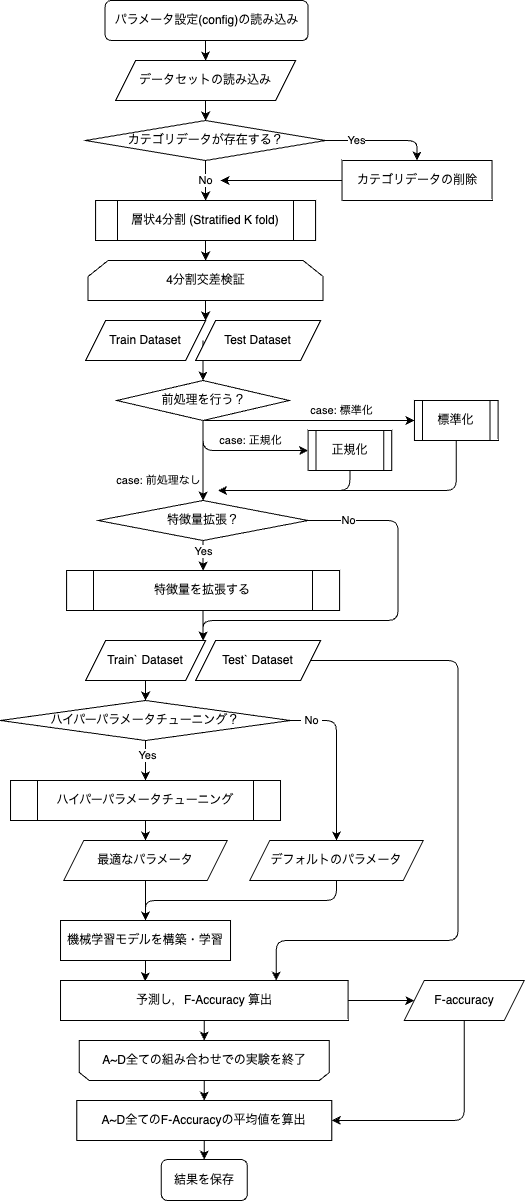
\includegraphics[width=0.6\linewidth\centering]{figures/ml-flow.png}
  \caption{実験の機械学習フロー}
  \label{fig:ml-flow}
\end{figure}
